\section{Introduction}
\label{sec:intro}

Vocabulary learning is an important part for both native and 
foreign language learning~\cite{grabe1991current,alqahtani2015importance} 
and has been shown to be useful for text readability assessment~\cite{nation2001learning,manyak2009english,qian2002investigating}. 
% \KZ{Give example of word classification in both English and German here.}
%Vocabulary knowledge is considered to be of great significance in both first language and second language studies~\cite{grabe1991current}, and has been indicated to be one of most useful features for text readability assessment~\cite{nation2001learning,manyak2009english,qian2002investigating}. 
%In particular, if the word difficulty is given during the second language learning, 
%%for example, for students who study English as a foreign language, 
%this can be useful for foreign language learners learning by stages and also be helpful for teachers setting tutorials and examinations.
%%\JQ{The sentence is too long}
%Therefore word difficulty has been paid much attention in standardized language tests which are used to measure the foreign language proficiency of non-native speakers.
Classifying words into different difficulty levels is essential for language education and there exist a number of word difficulty standards targeting different group of population.
% \KZ{Give example of word classification in both English and German here.}
%Core vocabulary of English for different grades is also the focus of the studies.
%For example, Kaplan and BerLiner Platz are famous language examination educational institutions for English and German.
%The compilation of vocabulary books plays an important role in teaching materials of both institutions.
For example, the compilation of vocabulary books plays a key role in teaching materials of Kaplan and BerLiner Platz. Both of them are famous language examination educational institutions for English and German.

Traditionally, the classification of words has been manually done by
educational or linguistic experts, which is a costly and  time-consuming
process. For example, the Common European Framework of 
Reference for Languages  (CEFR)~\cite{little2006common,little2011common}, 
an international standard for describing language ability, is the result 
of over 20-year work by Council of Europe to define the different language standards including the word difficulty. 
Such efforts cannot scale to less popular languages that are lack of required resources and expertise, and cannot keep up with the increasingly fast changes in vocabulary in today's world.

%and this has several pitfalls: time consuming, failing to catch up with dynamic changes of words, limited professional knowledge and coverage of foreign resources, etc. 
%%The development of language learning criteria and corresponding core vocabulary is empirical and time-consuming, 
% 
%Even for the educational institutions, the design of vocabulary books for foreign language tests are the contribution of years of teaching experience from educators. 
%%However, for such special tests to measure the English language ability, the number of their core vocabulary is limited. 
%However, the core vocabulary for such a special standard is limited, which can not meet the requirements of thorough learning.
%Generally, linguists and educationists devote themselves into the development of a wider size of vocabulary set 
%%based on core vocabulary 
%with the help of language criteria and specific environment of language examinations 
%%Such an experiential work is time-consuming and  
%which is time-consuming and labor-intensive.
 %effort-consuming% 
% labor-intensive which needs people with professional knowledge especially educational background to finish.\JQ{"Such .... finish." can be deleted}
%, but not universal and has poor generalization ability. 
%Unfortunately, because this is a skillful job,
%As a result of being such a technical task, 
%it is not easy
%% to update as the social environment and language usage change
%to update the word list with the change of the social environment and language usage.
%%What's more,
%%for language that is used by a small number of people, due to the lack of effective systems and methods and the limited coverage rate of foreign resources, it may make it  longer and much harder to study the word difficulty.
%Moreover, it is much harder to study the word difficulty for minority languages due to the lack of effective methods and limited resources.

%\KZ{Some recent attempts were made to classify words by difficulty computationally. These attempts were primarily restricted to using word frequency as a sole feature... And their main disadvantage is... illustrate using an example.}
%Some recent attempts were made to classify words by difficulty computationally. 
Some previous researches focused on the analysis of features that influence vocabulary knowledge.
Most attempts were restricted to using word frequency as a sole feature.
For example, some researches explored the correlations between the 
word frequency values and word difficulty ranks and showed that 
word frequency is highly correlated with word difficulty~\cite{breland1996word,ryder1988relationship,chang2018learning}.
However, frequency isn't the only critical feature in 
word difficulty classification and prediction.  
%People usually think the words often used are not complicated, but some words that are not commonly used may be also very simple.
%It is common sense that the more frequent the words, the simpler they are.
%But even in a very comprehensive corpus, there are still exceptions.
Although it is common sense that the word difficulty 
has negative correlation with its frequency, there are always 
exceptions and regarding frequency as the only critical features 
is not persuasive for this task. The following is a counter-example.
Figure \ref{fig:freqeg}
displays the relationship between some English word frequency and their difficulty levels in CEFR where words are divided into 6 difficulty levels.
%\SY{Can the figure be clearly understood???}
%several words with their frequency in COCA and its word difficulty level in CEFR in which words are divided into 6 categories according to the increase in difficulty.
%The difficulty of words as the frequencies decrease is observed in Figure \ref{fig:freqeg}(a). \JQ{delete}
%In the ideal state, the lower the frequency, the higher the word difficulty, and there should be a gradually dropping fold line.
%We hope a smooth descending line in Figure \ref{fig:freqeg}(a), but the polyline shows there are still some easy words with low frequency.
The blue polyline in Figure \ref{fig:freqeg} shows there are still some 
easy words with low frequency, which contradicts with the universal considered
smoothing decline line.
%Figure \ref{fig:freqeg}(a) shows that even if the word difficulty gradually rises as the frequency of the word decreases, there are still quite a few words with low frequency that are very simple.\JQ{what is the percentage of the words that do not follow the common sense rule?}
Table \ref{tab:words} uses some unconventional examples to confirm this again.
%Some words related to polics or news such as ``revenue", ``ethnic'' and ``legislation'' have high frequencies even they are difficult in learning.
%We find some easy words in last three rows of \ref{fig:freqeg}(b) may have lower frequency because they only appear in some certain occasions or areas.

\begin{figure}[th]
	\centering
	%	\epsfig{file=pic/bitri.eps, width=0.9\columnwidth}
	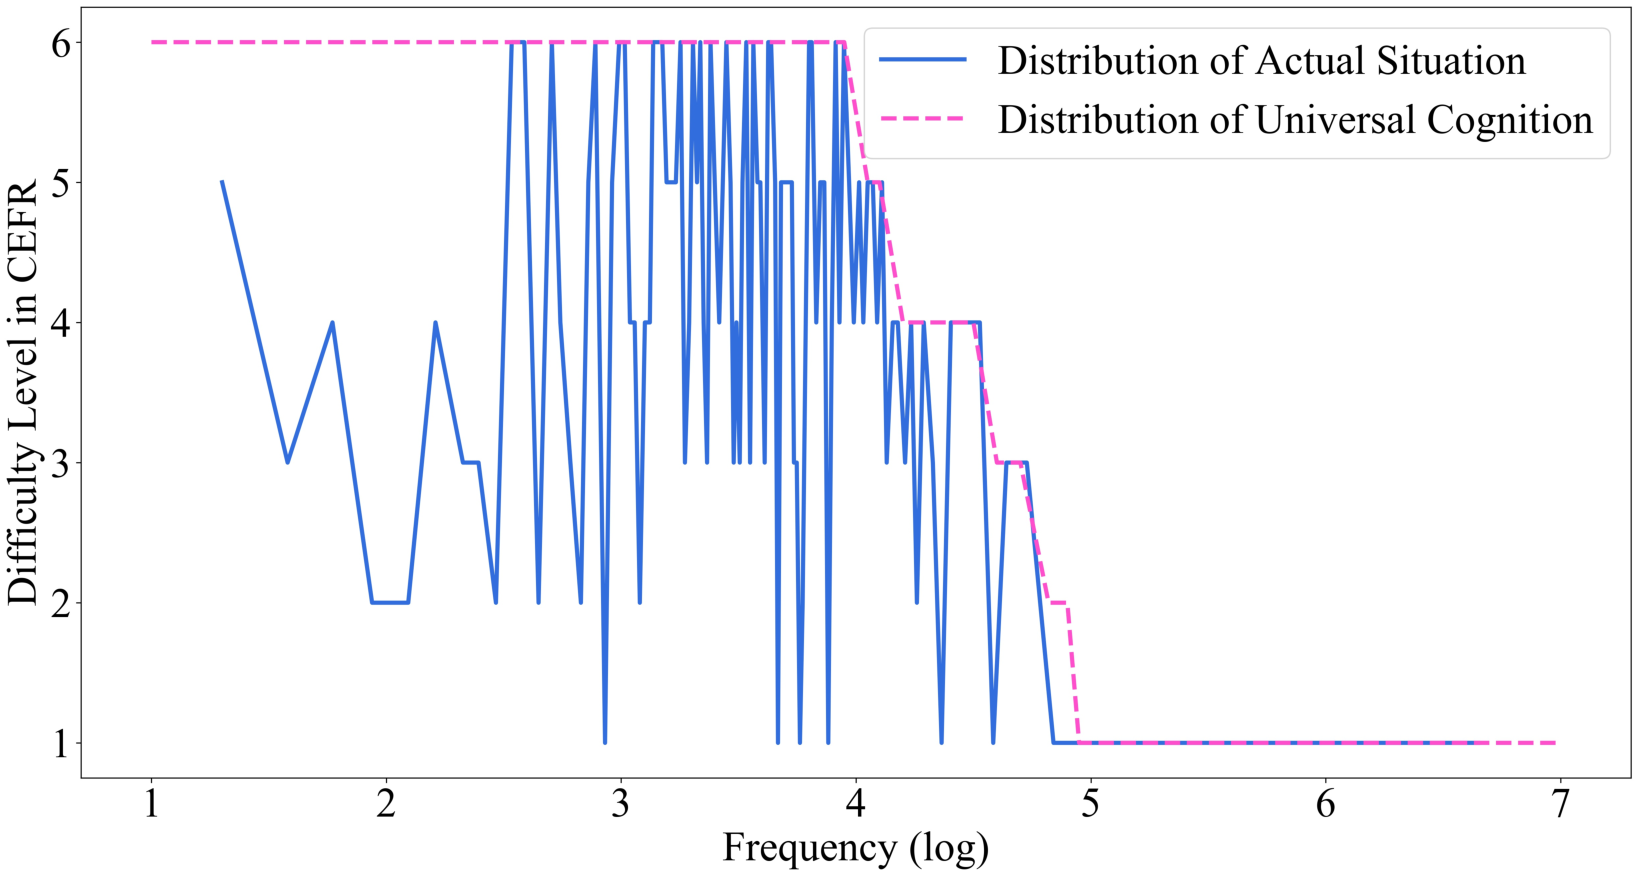
\includegraphics[width=\linewidth]{pic/example.pdf}  
	%\caption{Overview of proposed model, which shows how Attention Filter Mechanism (ATTF) works when decoding $Y_i$.}
	\vspace{-0.25cm}
	\caption{\label{tab:freqeg} The relationship between word's difficulties and their frequency.}
	\label{fig:freqeg}
\end{figure}
\vspace{-0.5cm}
\begin{table}[th]
	\scriptsize
\begin{center}
		\begin{tabular}{ccc}
		\hline
		\textbf{Word} & \textbf{Frequency in COCA} & \textbf{CEFR LEVEL} \\ \hline
%		revence & 24255 & 5 \\ 
		ethnic & 23752 & 5 \\ 
		legislation & 20186 & 6 \\ 
		queen & 31 & 2 \\ 
		jazz & 26 & 2 \\ 
		vegetable & 24& 1 \\ \hline
	\end{tabular}
\end{center}
\vspace{-0.25cm}
\caption{\label{tab:words} Examples of words with COCA frequency and CEFR level.}
\end{table}

%Some educational research also examine the features of words which contributes to the ease or difficulty of vocabulary knowledge, such as frequency, domain specificity, semantic relatedness, morphological relatedness, etc~\cite{EH2019analysis}. 
%Some educational research also 
%Other attempts examines the binding features that influence the word difficulty, such as the binding of frequency, domain specificity, semantic relatedness, morphological relatedness and etc~\cite{EH2019analysis} or the binding of word frequency, length, the number of syllables and the number of consonant clusters in a word~\cite{koirala2015word}.
Others attempted compound features that contribute to 
the word difficulty. 
Hiebert et al.~\shortcite{hiebert2019analysis} used the combination of frequency, domain specificity, semantic relatedness, 
morphological relatedness and etc. 
%Koirala~\shortcite{koirala2015word,culligan2015comparison} 
Others have used  the combination of word frequency and orthographic features which includes length, the number of syllables, the number of consonant clusters and the number of phonemes in a word~\cite{koirala2015word,culligan2015comparison}.
%\KZ{You just talked about frequency, why mention it again here? ``Research'' is an uncountable noun. Also rephrase the following sentence. 
%I don't understand what it means.}
%The research mentioned above drawn the conclusion by continuous observation and adjustment which need to examine students' performance on vocabulary assessments.
%However most research focus on the study of vocabulary size a student should master in different grades.
Still, most of the above research focus on the linguistic theory of
word difficulty and has not developed 
%these are mainly the theoretical research, 
effective ways to computationally generate or predict the 
words with varying difficulty.
Therefore these methods still don't scale. 
%\SY{Anything else?}
%As far as we know, no one has achieved end-to-end word difficulty classification based on comprehensive suite of features. 
%\KZ{You have to identify what's the weakness or shortcoming of the above approach and not say that they are bad because they haven't use d a comprehensive suite of features! That's not their fault. Maybe their limited set of features will work?? The key is, what inspired us to use the new features that were not attempted previously by others.}

%Natural language processing (NLP) methodologies
%have been widely adopted in linguistic area and greatly enhanced predictive accuracy in lots of tasks. 
%We hope NLP and machine learning methodology can do a favor to classify the word difficulty and extend the core vocabulary set  based on a specific corpus or application scenario instead of artificial labor.
%\JQ{Lack of a conclusion of technical challenges. And the two paragraph}
%\KZ{is it true previously no other methods have used a large open-domain corpus to extract features? But they have used frequencies before, and frequency must be measures from a large corpus as well?} 
%\KZ{To address the technical challenges faced by previous approaches, we proposed to extract features from a large open-domain text corpus for the word difficulty classifier.}
To address the technical challenges faced by previous approaches, 
we propose to extract features from large open-domain text corpora 
for representing word difficulty.
%Therefore, we proposed a method which we can 
%extend the offical core vocabulary 
%predict the difficulty of a word more accurately with the help of a huge corpus of articles, making it easier to update the core vocabulary list.
%\KZ{What standard you use or what detailed corpus you use is independent from
%the framework and they should not be discuss here or in the approach section.
%Rather they should be discussed only in the eval section.}
%First, we choose a classified vocabulary for both English and German
%from the Common European Framework of Reference for Languages  (CEFR)~\cite{little2006common, little2011common} as the ground truth.
%Second, we learn the features of words under a big corpus such as The New York Times Annotated Corpus~\cite{Evan2008newyork} and Gutenberg Dataset~\cite{lahiri:2014:SRW}, focusing on the morphological features, syntactic features and semantic features. 
%%Core vocabulary from CEFR are labeled into 6 levels as A1, A2, B1, B2, C1 and C2. %shown in Table \ref{tab:CEFR}%. 
%Features describing the word difficulty are listed in Table \ref{tab:features} and Section \ref{sec:approach}. 
%Then, logistic regression and multi-layer perception are implemented to predict the word difficulty.
%Finally, the results in different corpora environments show that semantic features generated by word embedding are the most effective.
%When the same analytical method is applied to the study of German word difficulty, we obtain the same result, which proves that our method is robust and can be widely applied to multiple languages. 
In order to explore whether our feature engineering method can be generalized 
to different corpus environments and language environments,
%in different corpus environments for the same language environments and different language environments, 
we conduct experiments on both English and German corpora.
We choose the authoritative word lists leveled by difficulty for both 
English and German as the ground truth.
%Then, we extract the features of words from a large open-domain corpus for each sub-experiment.
%Finally, various classifiers are used to predict the word difficulty level.\JQ{too steps, maybe not too steps}
In order to measure the effectiveness of extracted features for this task, we do experiments on both the word difficulty level classification task and the word-pair difficulty ranking task.

%the difficulty of the words, both the word difficulty level classification task and the word pairs difficulty ranking task are chosen.
The results in different English corpus environments 
show that semantic features generated by word embedding are most effective.
%When the same analytical method is applied to the study of German word difficulty,\JQ{
When applying to German, we obtain the same result.
It shows that our method is robust under different corpus environments 
and can be applied to different languages. 

%\begin{table*}[]
%	\begin{tabular}{|c|c|c|}
%		\hline
%		\textbf{Level} & \textbf{Description}                          & \textbf{Examples}                  \\ \hline
%		\textbf{A1}    & Breakthrough or beginner                      & birthday, he, because              \\ \hline
%		\textbf{A2}    & Waystage or elementary                        & bookshelf, everybody, shorts       \\ \hline
%		\textbf{B1}    & Threshold or intermediate                     & nightlife, spectacular, sunshine   \\ \hline
%		\textbf{B2}    & Vantage or upper intermediate                 & literally, acquire, approval       \\ \hline
%		\textbf{C1}    & Effective operational proficiency or advanced & bacteria, selfishness, untouched   \\ \hline
%		\textbf{C2}    & Mastery or proficiency                        & contraception, omplexion, narrator \\ \hline
%	\end{tabular}
%	\caption{\label{tab:CEFR} The Description of CEFR Level and Example Words.}
%\end{table*}

%\begin{table}[th]
%	\begin{center}
%		\scriptsize
%		\begin{tabular}{|l|l|}%{|p{7cm}|rl|}
%			\hline
%			\textbf{Feature}& \textbf{Description} \\
%			\hline
%			Frequency&Occurring times in corpus of one word.\\
%			\hline
%			length& Length of one word.\\
%			\hline
%			Pronunciation& Word's syllable vector\\
%			\hline
%			uPOS&Word's universal part-of-speech value.\\
%			\hline
%			xPOS&Word's treebank-specific \\
%			&part-of-speech value.\\
%			\hline
%			Bigram Vector&Word's bigram transform.\\
%			\hline
%			Trigram Vector&Word's trigram transform.\\
%			\hline
%			Bigram Probablilty&Word's coherence probability \\
%			&calculated by bigram form.\\
%			\hline
%			Trigram Probablilty&Word's coherence probability\\
%			&calculated by trigram form.\\
%			\hline
%			Embedding Vector& Word Vector obtained by Word2Vec.\\
%			\hline
%			Type of Dependency&Type of dependency obtained by\\
%			& constituency parsing.\\
%			\hline
%		\end{tabular}
%	\end{center}
%	\caption{\label{tab:features} Features from Different Levels to Describe Word Difficulty.}
%\end{table}

% \usepackage{multirow}

%\begin{table*}[ht]
%	\centering
%	\scriptsize
%	\begin{tabular}{|l|l|l|}
%		\hline
%		\textbf{Feature}         & \textbf{Feature}  & \textbf{Description}   \\ \hline
%		Frequency                      & Frequency        & The number of a word's occurrences in the corpus                  \\ \hline
%		\multirow{4}{*}{Morphological} & Length              & The number of characters in a word                                     \\ \cline{2-3} 
%		& Syllable Vector      & The bag-of-syllables representation of a word                                \\ \cline{2-3} 
%		& N-gram Vector            & N-gram transform of a word.                              \\ \cline{2-3} 
%		& N-gram Probability    & \tabincell{l}{A probabilistic language model based on n-gram at word level.} \\ \cline{2-3} \hline
%		\multirow{2}{*}{Syntactic}     & POS Tag              & Word's treebank-specific part-of-speech value.           \\ \cline{2-3} 
%%		& uPOS                      & Word's universal part-of-speech value.                   \\ \cline{2-3} 
%		& Type dependency         & \tabincell{c}{Universal dependencies obtained by constituency parsing. }   \\ \hline
%		Semantic                       & Word embedding       & Pre-trained word vectors by Skip-gram model                 \\ \hline
%	\end{tabular}
%	\vspace{-0.25cm}
%	\caption{\label{tab:features} Multi-faceted features describing the word difficulty.}
%\end{table*}

Our contributions are summarized as follows:
\begin{enumerate}
	\item To the best of our knowledge, we are the first to classify and compare words by the difficulty using multi-faceted features.
	We discover that semantic features generated by word embeddings are most important in determining the words difficulty (Section \ref{sec:embedding}).
	\item Our approach of using multi-faceted features to measure word difficulty outperforms the the frequency-only baseline and our accuracy of the word classification and word-pair ranking tasks are very close to the human baseline(Section \ref{sec:res}).
	\item Our method shows robustness against different corpus environments of the same language and is capable for predicting word difficulty in different languages, making it easier in updating the vocabulary lists for different word difficulty levels in new languages or 
	%	teaching conditions 
	educational environments (Section \ref{sec:embedding}, \ref{sec:res}).
\end{enumerate}

In Section \ref{sec:approach}, multi-faceted features that represent the word difficulty are discussed. 
In Section \ref{sec:eval}, we introduce the process of the experiment and give an analysis of the results.
Section \ref{sec:related} is the related work and Section \ref{sec:conclude} comes the conclusion.
